\documentclass[12pt,a4paper]{article}
\usepackage[utf8]{inputenc}
\usepackage{graphicx}
\usepackage[a4paper, textwidth=15cm, textheight=23cm]{geometry}
\usepackage[section]{placeins}

\renewcommand{\contentsname}{Gliederung}
\renewcommand{\figurename}{Fig.}

\title{Praxisprojekt: PharoThings-Connectivity SS19}
\begin{document}
	\begin{titlepage}
    
\includegraphics[width=0.4\textwidth]{th_logo.png}
    ~\\[2.5cm]
    \begin{center}
    \textbf{\huge Verbindungskonfiguration von PharoThings auf Raspberry Pi durch Android App}\\[0.5cm]
    {\Large Praxisprojekt Sommersemester 2019}
    \vfill
    \end{center}
    ~\\[2.0cm]
    \begin{flushright}
    {\large Jan Phillip Kretzschmar \it{(jan@2denker.de)}}\\[0.1cm]
    ~\\[1.0cm]
    {\large Betreuer (Zweidenker GmbH):}\\[0.1cm]
    {\large Christian Denker \it{(christian@2denker.de)}}
    ~\\[0.5cm]
    {\large Betreuer (TH Köln):}\\[0.1cm]
    {\large Prof. Christian Kohls}\\[0.1cm]

	~\\[1.0cm]
    {\large 30. Juni 2019}
	\end{flushright}
    \end{titlepage}
    \tableofcontents
    \pagebreak
    \section{Expose}
    Pharo ist eine auf Smalltalk basierende objektorientierte und dynamisch getypte Programmiersprache,
    welche gleichzeitig ihre eigene live Entwicklungsumgebung mit mächtigen Debugging-Tools ist.\footnote{http://pharo.org/}
    PharoThings bietet eine reduzierte Platform für  Internet of Things(IoT), sodass eine Ausführung von Programmen auf Kleinstcomputern möglich ist.
    Um keine Kompromisse im Bereich der Entwicklungsumgebung machen zu müssen, kann über Remote Debugger auf live Programme zugegriffen werden.
    Dadurch ist lediglich die Ausführung auf das IoT Gerät ausgelagert. PharoThings bietet in Verbindung mit WiringPi eine Platform für Raspberry Pi,
    auf der Board Modeling simpel möglich ist.\footnote{https://github.com/pharo-iot/PharoThings}
    Für die Erstkonfiguration und Verbindungskonfigurationvon PharoThings auf Raspberry Pi ist es aktuell nötig,
    diese Konfiguration z.B. der WLAN-Verbindung durch einen Computer vorzunehmen.
    Um die Pharo Things Laufzeitumgebungen als IoT-Geräte simpel nutzen zu können, ist es nötig,
    die Konfiguration der Installationen und Geräte zu vereinfachen. Dabei soll eine Android App diesen Vorgang übernehmen:
    \begin{enumerate}
        \item Erkennen und Auflisten von IoT-Geräten in der Nähe. Die zu verwendende Kommunikationstechnologie ist dabei zu evaluieren.
        \item Verbindungsaufbau zu ausgewähltem IoT-Gerät
        \item IoT-Gerät erhält Hostnamen, WLAN-Konfiguration, Beacon Intervall, etc.
        \item Eventuelle Verbindungsprobleme der erst WLAN-Verbindung werden über die bestehende Verbindung zurückgemeldet
        \item Pharo Things-Installationen im aktuellen WLAN werden aufgelistet.
    \end{enumerate}
    Um diesen Vorgang umsetzen zu können, werden drei Komponenten implementiert:
    \begin{enumerate}
        \item Ein Protokoll muss definiert werden, welches die Kommunikation zu PharoThings Instanzen zur Konfiguration festlegt.
        Weiterhin muss festgelegt werden, in welcher Art und Weise ein Beacon-Signal im WLAN von den Installationen gesendet wird.
        Um das WLAN nicht zu überlasten, empfiehlt es sich diese Nachrichten kurz zu halten. Es ist zu evaluieren,
        ob sich Installationen auch gegenseitig erkennen können, sodass ein gebündelter Beacon gesendet werden kann.
        \item Eine Android App, welche den Nutzer durch den beschriebenen Vorgang leitet, muss implementiert werden.
        Der Fokus hierbei liegt darin, diesen Vorgang mit möglichst wenig Nutzerinteraktion durchzuführen.
        \item Eine Anwendung in PharoThings muss erstellt werden, welche das Protokoll implementiert
        und basierend darauf sich in einem WLAN einwählen kann und ein Beacon-Signal in diesem WLAN sendet.
    \end{enumerate}
    Das Projekt wird mit Unterstützung der Zweidenker GmbH durchgeführt.
    \section{Mögliche Kommunikationstechnologien}
    Ein Ad Hoc Netzwerk bietet im Allgemeinen die Möglichkeit {\it peer to peer} (p2p) Verbindungen zwischen Geräten dezentralisiert aufzubauen.
    Geräte können hierbei selbstständig eine Netzwerkverbindung untereinander aushandeln. Da solche Verbindungen nur dann sinnvoll sind,
    wenn es Daten gibt, die nur zwischen den beiden verbundenen Geräten ausgetauscht werden müssen, ergibt ein solches Netzwerk meist nur
    im Bezug auf eine tatsächlliche Anwendung Sinn. Die erweiterte Definition des Ad Hoc Netzwerks
    bezieht somit alle Netzwerkschichten des OSI-Modells mit ein.\cite[S.23]{Sikora}
    Obwohl das OSI-Modell vor Allem auf Ethernet und WLAN ausgelegt ist, lässt sich die Definition des Ad Hoc Netzwerks
    dennoch für weitere Kommunikationstechnologie übernehmen, da diese ebenfalls p2p Verbindungen aufbauen können.
    Optimalerweise sollte es möglich sein die bestehenden WLAN-Verbindungen beider Geräte während einer p2p Verbindung beibehalten zu können.
    Für Kommunikationsmedien in diesem Projekt fallen einige Beschränkungen an: 
    \begin {enumerate}
    \item {\it Reichweite:}
    Netzwerke werden oft nach ihrer Reichweite klassifiziert. Dabei gibt es die geläufigen Bezeichnungen Local Area Network (LAN),
    Metropolitan Area Network, Wide Area Network und Global Area Network, die in ihrer Klassifizierung von Gebäuden zu einer Globalen Reichweite übergehen.
    Üblicherweise verbinden höhere klassifizierte Netzwerke niedriger klassifizierte Netzwerke miteinander. Im Bereich der Drahtlosnetzwerke gibt es jede
    dieser Klassen ebenfalls als Drahtlos-Variante: WLAN, WMAN, WWAN und WGAN, es kommen jedoch noch zwei in ihrer Reichweite kleinere Netzwerke hinzu,
    das Wireless Body Area Network und das Wireless Personal Area Network. Übliche Einsatzgebiet des WBAN sind im medizinischen Bereich zu finden,
    aber auch Near Feald Communication fällt in diese Kategorie. Unter die Klassifizierung des WPAN fällt unter anderem Bluetooth,
    für dieses Projekt sind somit Funknetzwerke der untersten drei Kategorien WBAN, WPAN und WLAN oder deren kabelgebundenen Derivate interessant.\cite[S.17]{Lueders}
    \item {\it Unterstützung in Android Smartphones:}
    Damit eine große Anzahl an potentiellen Nutzern angesprochen werden kann, muss die Verbindungsschnittstelle von Smartphones unterstützt werden.
    Für dieses Projekt wird dabei nur Android betrachtet.
    Aktuelle Smartphones bieten im Allgemeinen zur Zeit die vier Schnittstellen {\bf USB, NFC, Bluetooth und Wi-Fi},
    über die sich Verbindungen zu Geräten in der näheren Umgebung aufbauen lassen.
    \item {\it Hardware an IoT Geräten:}
    Als IoT Gerät dient in diesem Projekt ein Raspberry Pi.
    In den Varianten {\it Model 3 B, Model 3 B+ and Model Zero W} bietet Dieser USB, Bluetooth und Wi-Fi als mögliche Schnittstellen.
    Durch die Verwendung der GPIO-Pins ist es außerdem möglich, ein NFC-Modul anzubinden,
    jedoch würde Dies die später nutzbaren Pins unerwünscht einschränken.
    Weiterhin bietet der Raspberry Pi ein vollständiges Betriebssystem mit Benutzeroberfläche, jedoch soll eine Internetverbindung
    ohne Peripherie am Raspberry Pi konfiguriert werden können. 
    \end {enumerate}

    \subsection{Kommunikation über WLAN}
        Der IEEE802.11 Standard siedelt sich im OSI-Modell lediglich in der Physical Layer und Data Link Layer an. Ihr eigentlicher Sinn ist es,
        IP-Pakete der Network Layer im gleichen Maße wie ein LAN übertragen zu können.
        Die Definition des Wireless LAN unterscheidet sich jedoch vom LAN Standard dahingehend, dass eine vollständig eigene Physical Layer geschaffen wurde,
        da das Übertragungsmedium andere Restrikitionen besitzt. Die Data Link Layer setzt sich für WLAN größtenteils aus drei Teilen zusammen.
        Die Logic Link Control nach 802.2 und das Bridging nach 802.1 sind mit LAN identisch, um der Network Layer eine einheitliche Schnittstelle unabhängig des Übertragungsmediums zu bieten.
        In der Data Link Layer unterscheidet sich lediglich der Media Access Control (MAC).\cite[S.311]{Sauter}
        Dieser regelt im Fall von WLAN den Zugriff auf das Übertragungsmedium durch unterschiedliche Wartezeiten zwischen Frames und die Reservierung des Mediums zum Senden von Frames.
        Da das MAC-Protokoll zudem die Addressierung von Geräten ermöglicht, bietet es ebenfalls bereits die Möglichkeit, Broadcasts zu senden.
        Um die hohe Fehleranfälligkeit eines Drahtlosnetzwerkes für höhere Schichten zu reduzieren, wird jedes Frame vom Empfänger bestätigt.\cite[S.325-327]{Sauter}
        
        Ein Netzwerk nach 802.11 kann hierbei entweder im Infrastruktur Modus, in dem alle Geräte ausschließlich mit einem Access Point kommunizieren,
        oder im Ad Hoc Modus, welcher die direkte Kommunikation zwischen Geräten erlaubt, betrieben werden.\cite[S.82]{Sikora}
        Ein Verbindungsaufbau ist für eine p2p Verbinung entweder durch eine konkrete Implementierung des Ad Hoc Modus oder
        im MAC-Protokoll zu ersuchen.

        Unter dem Markennamen Wi-Fi\textsuperscript{TM} werden 802.11-kompatible Geräte zertifiziert.\cite[S.80]{Sikora}
        Für den Ad-hoc Modus nach 802.11 wurde dabei Wi-Fi Peer-to-Peer (Wi-Fi Direct)\textregistered\cite{wifiDirect} als ein universeller Standard definiert.
        Durch Wi-Fi Direct ist es jedoch ebenfalls möglich, einen Verbindungsaufbau in der {\bf Application Layer} des OSI-Modells anzusiedeln.
        Dazu bietet diese Spezifikation neben dem normalen Peer-To-Peer Modus die Möglichkeit, Services anzubieten und zu finden, bevor eine Verbindung etabliert werden muss.
        Grundlage für diese Services bilden dabei DNS Service-Discovery (DNS SD) und Universal Plug and Play (UPnP).
        DNS SD ist die Weiterentwicklung von Apple Bonjour und wird größtenteils genutzt um eine Zero-Configuration Service Discovery von beispielsweise Netzwerkdruckern zu ermöglichen. Da UPnP im Gegensatz zu DNS SD auch die Kontrolle über die Services übernimmt, besitzt es einige Verwundbarkeiten. Man kann es jedoch ähnlich zu DNS SD lediglich dazu benutzen, Services zu ernennen.\cite{Esnaashari}
    
        \paragraph{Nutzung unter Android}
        Im Gegensatz zu Apple AirPlay kann für eine App nicht auf Gerätetreiber-Ebene entwickelt werden. Um MAC in Linux verwenden zu können, ist es nötig, Sockets mit dem Attribut {\bf SOCK\_RAW} zu öffnen,
        um eigene MAC-Pakete senden zu können. Solche Sockets können jedoch nur mit der Berechtigung {\bf CAP\_NET\_RAW} erstellt werden.\cite{linuxPacket}
        Unter Android fällt diese Berechtigung mangels Granularität root zu, wodurch diese Lösung unpraktikabel wird,
        wenn eine möglichst große Nutzergruppe angesprochen werden soll.\cite{androidRights}
        Android bietet jedoch ab API 14 die Möglichkeit, sich über WI-Fi Direct als möglicher peer anderen Geräten zu präsentieren und
        p2p Verbindungen aufzubauen, sowie Services bereitzustellen und zu erkennen.
        Android stellt diese p2p Funktionalität als {\it WifiP2PManager} bereit. Ein kurzer Test mit zwei Android Geräten hat dabei ergeben,
        dass dieser bestehende Wi-Fi-Verbindungen während der Service Discovery beibehält.\cite{test-repository}
        Ein ähnlicher Ansatz, in dem Wi-Fi Direct genutzt wird, um ein Ad Hoc Netzwerk aufzubauen findet sich in \cite{Aneja}.

    \subsection{Kommunikation über Bluetooth}
        Die grundlegenden Komponenten von Bluetooth sind im Standard IEEE802.15.1 als {\it Bluetooth Core} definiert. Anwendungen können über diesen Kern oder speziellere Protokolle Bluetooth
        Verbindungen zu anderen Geräten aufbauen.\cite[S.228]{Lueders}
        Um Daten über Bluetooth senden zu können, muss eine Verbindung zwischen den beiden Geräten aufgebaut werden. Für diese Verbindung ist es nötig,
        dass sich die entsprechenden Geräte zunächst koppeln. Zum Koppeln verfügbare Geräte werden hierbei durch eine sogenannte Inquiry, welche erreichbare Geräte auffordert,
        sich zu identifizieren, aufgelistet. Da nun die Adresse des zu koppelnden Gerätes bekannt ist, kann zu diesem eine Koppelung angefragt werden, was als Paging bezeichnet wird.
        Die Kopplung dient dabei dem Austausch der Frequency Hop Sequenzen, welche festlegt, wann auf welcher Frequenz Pakete gesendet werden, sowie dem Pairing von Geräten, welches sicherstellt,
        dass das richtige Gerät gekoppelt wird und Schlüssel zur Authentifizierung und Verschlüsselung überträgt.\cite[S.402f.]{Sauter}

        Sobald eine Verbindung zwischen den Geräten aufgebaut wurde, können Daten bidirectional übertragen werden, indem ein Bluetoothkanal, anders als WLAN, in Zeitslots unterteilt wird.
        Die alleinige Kontrolle, welches Gerät wann Daten senden darf, hat dabei das Mastergerät des Netzes. Das Gerät, welches den Verbindungsaufbau angefragt hat,
        agiert dabei als Master und bis zu sieben weitere Geräte können als Slave in einem Piconetz verbunden sein.\cite[S.379f.]{Sauter}

        Für bestimmte Anwendungsfälle gibt es spezielle Protokolle, welche generische Lösungen dieser Fälle bieten.
        So ermöglicht das Service Discovery Protocol (SDP) den Informationsaustausch über verfügbare Dienste der Kommunikationspartner,
        Radio Frequency Communications (RFCOMM) kann serielle Schnittstellen abbilden und das Object Exchange Protocol (OBEX) kann Datenobjekte über RFCOMM übertragen.\cite[S.229]{Lueders}
        SDP erlaubt nicht nur das Auflisten von verfügbaren Diensten des Verbindungspartners, sondern auch das Suchen von einem bestimmten Dienst auf erreichbaren Geräten,
        es kann dabei jedoch keinen Zugriff zu den Diensten bereitstellen oder die Verfügbarkeit der Dienste auf den erreichbaren Geräten angeben.\cite[S.395f]{Morrow}

        Bluetooth lehnt sich mit dem {\it Bluetooth Core} nur lose an das OSI-Referenzmodell an, da nicht jedes Element des Bluetoothstacks sich sauber einer OSI-Schicht zuordnen lässt.
        Die oben vorgestellten Protokolle wie SDP oder RFCOMM siedeln sich jedoch in der {\bf Presentation Layer} an, da diese lediglich dazu gedacht sind,
        Daten leichter der Anwendung zur Verfügung stellen zu können.\cite[S.382]{Sauter}

        \paragraph{Bluetooth Low Energy}
        Als Teil des Bluetooth Standards ist Bluetooth Low Energy (LE) darauf ausgelegt, Daten mit einem möglichst geringen Energieverbrauch über die Bluetooth-Hardware zu übertragen.
        Dies wird ermöglicht, indem verbindungslose Broadcast, die Nutzerdaten enthalten können definiert werden, sowie aktive Verbindungen zwischen zwei Geräten auf eine kurze Übertragung von 6 Packeten pro Verbindungsevent limitiert werden. Verbindungsevents sind dabei durch ein wählbares Intervall zwischen 7.5ms und 4s von einander getrennt. Weiterhin beschränkt sich Bluetooth LE im Hinblick auf die Reichweite darauf, möglichst wenig Energie zu verbrauchen, da eine hohe Sendeleistung in einem hohen Energieverbrauch resultiert. Da sich die Sendeleistung jedoch pro Gerät konfigurieren lässt, ist die theoretische Reichweite ähnlich zu Bluetooth gegeben.\cite[S.7f.]{Townsend}

        \paragraph{Nutzung unter Android}
        Android stellt sowohl Bluetooth als auch Bluetooth LE als {\it BluetoothAdapter} bereit. Ähnlich zu Wi-Fi Direct  Android bietet ab API 5 bzw. API 18 die Möglichkeit, über Bluetooth als möglicher peer anderen Geräten zu präsentieren und
        p2p Verbindungen aufzubauen. Über Bluetooth LE können hingegen Services als Broadcasts bereitgestellt werden. Bluetooth in Verbindung mit Bluetooth LE lässt sich somit im Rahmen dieser Arbeit ohne Probleme auf Android benutzen.

    \subsection{Kommunikation über NFC}
        Die Near Field Communication (NFC)-Technologie basiert auf RFID-Systemen und erlaubt die Übertragung von Daten auf eine Distanz bis zu 10 Zentimeter.
        Grundlegend ist NFC in den Standards NFCIP-1 (ECMA-340) und NFCIP-2 (ECMA-352) definiert. Wie bei klassischen RFID-Systemen ist ein magnetisches Feld
        als Trägersignal der Daten definiert. Dieses magnetische Feld dient dazu, passiven Komponenten, die keine eigene Stromversorgung besitzen, auf Anfragen
        der steuernden Komponente zu antworten. Anders als RFID hebt NFC jedoch die strikte Trennung zwischen steuernder (Initiator) und gesteuerter (Target) Komponente auf, sodass
        jedes teilnehmende NFC-Gerät zumindest theoretisch beide Rollen übernehmen kann.\cite[S.89]{Langer} Rückwärtskompatibilität erreicht NFC,
        indem sowohl ein Reader-Writer-Modus, der die Kommunikation mit passiven RFID-Transpondern ermöglicht,
        als auch ein Card-Emulation-Modus, der die Kommunikation mit RFID-Lesegeräten erlaubt, definiert ist.\cite[S.99f.]{Langer}
        Als letzter Modus ist der hier relevante Peer-to-Peer-Modus, dazu in der lage, Daten zwischen zwei NFC-Geräten zu übertragen.
        Ähnlich zu Bluetooth lehnt sich auch NFC nur lose an das OSI-Modell an. Es gibt für NFC drei aufeinander aufbauende Protokollschichten.
        Die Bitübertragung ist in NFCIP-1 definiert und teilt sich in einen aktiven und passiven Modus. Der aktive Modus hebt sich dabei vom passiven Modus,
        welcher in seiner Funktionsweise äquivalent zum RFID-System ist, dadurch ab, dass das Trägersignal von beiden Kommunikationspartnern abwechselnd generiert wird.
        Die darauffolgende Schicht ist ein MAC Protokoll, welches den Zugriff auf das Übertragungsmedium sichert, indem geprüft wird, ob bereits ein Trägersignal existiert,
        bevor ein Gerät in den Initiator-Modus wechselt, andernfalls verbleibt es im Target-Modus.
        Die letzte Schicht bildet das Logic Link Control Protocol (LLCP), welches es beiden Kommunikationspartnern erlaubt, eine Datenübertragung zu initiieren.\cite[S91.f, S.97]{Langer}

        \paragraph{Nutzung unter Android}
        NFC wurde unter Android, verteilt über die API Versionen 9, 10 \& 14,  als {\it NfcManager} und {\it NfcAdapter} zur Verfügung gestellt. Im Gegensatz zu Wifi, wo lediglich Verbindungszustände als Broadcasts gemeldet werden, werden bei Nfc die gelesenen Daten als Broadcasts an alle zuhörenden Apps gesendet, wodurch sich eine gesicherte Verbindung nicht gewährleisten lässt.

    \subsection{Kommunikation über USB}
        Im Gegensatz zu den vorhergehenden Übertragungsmedien ist der Universal Serial Bus (USB) eine kabelgebundene Schnittstelle. Aus der maximalen Kabellänge von 5 Metern
        ergibt sich somit auch die maximale Reichweite der Technologie. USB ist primär darauf ausgelegt, (Peripherie-)Geräte an einen Host anzuschließen.
        Der Host stellt hierbei eine minimale Versorgungsspannung auf dem Bus bereit, sodass Geräte sich beim Host registrieren können und eine höhere Stromversorgung anfordern können.
        Weiterhin übernimmt der Host zwangsläufig auch die Kontrolle über die Verbindung, da Geräte zu jedem Zeitpunkt physisch vom Bus entfernt werden können, sodass Hot-Plug-and-Play
        möglich wird. \cite[S.21-24]{Kelm}
        Da USB eine möglichst breite Anzahl an Geräten zu unterstützen versucht, ist es nötig in den meisten Fällen einen Treiber auf dem Host bereitzustellen, sodass Anwendungen mit dem USB-Gerät kommunizieren können.\cite[S.197]{Kelm}

        \paragraph{Nutzung unter Android}
        Durch das Android Open Accessory Framework, welches ab API 10 angeboten wird, ist es möglich, mit einem Android-Gerät über USB zu kommunizieren und dabei als Host zu agieren. Es ist hierbei jedoch nötig einen Treiber auf Host-Seite zu schreiben, um dieses Framework nutzen zu können.\cite{AOA}

    \subsection{Evaluation der Übertragungsmedien}
    Alle vorgestellten Schnittstellen, außer USB, lassen sich unter Android, wie in \cite{test-repository} zu sehen, mit ähnlichem Aufwand anbinden.
    Da für USB ein Treiber auf Hostseite nötig ist, der AOA implementiert, ist der Aufwand wesentlich höher im Vergleich zu den restlichen Schnittstellen.
    Unter Pharo wurde bisher keine dieser Kommunikationskanäle angebunden,
    jedoch lassen sich bereits Sockets in Pharo nutzen und damit MAC-Pakete versenden.
    Da WLAN die größte Reichweite im Vergleich zu den restlichen gezeigten Technologien bietet, stellt sich hierbei ebenfalls Wi-Fi Direct als sinnvollste Schnittstelle heraus.
    Da nicht jedes Android-Gerät Wi-Fi Direct unterstützt, ist es jedoch sinnvoll, die Implementierung der Konfigurationsschnittstelle so zu kapseln,
    dass sie auch über andere Kanäle angesprochen werden kann.
    
    Der Austausch über Bluetooth über verfügbare Dienste der Geräte ist erst nach einer vollständigen Kopplung und Verbindung möglich.
    Dadurch ist ein Filtern der verfügbaren Bluetooth Geräte zur Auswahl durch den Nutzer nur über den Namen oder die Adresse des Gerätes möglich.
    Im Gegensatz dazu ermöglicht Bluetooth Low Energy eben genau die gleiche Funktionalität wie Wi-Fi Direct, indem Daten ohne eine aktive p2p-Verbindung übertragen werden können. Es sollte somit Bluetooth nur in Kombination mit Bluetooth Low Energy genutzt werden.

    Um dem Nutzer möglichst einfach erreichbare Geräte zeigen zu können, ist es wünschenswert, dem Nutzer wenig bis keinen Aufwand bei der Anbindung des Gerätes über die Übertragungsmedien zu geben.
    Wi-Fi Direct bietet hierbei mit DNS SD eine Lösung, um Dienste ohne Konfiguration auf Seite von Client-Geräten vorzustellen, die keinerlei Aufwand für den Nutzer bedeutet.
    Bluetooth Low Energy bietet ebenso die Möglichkeit, Beacon-Signale mit Nutzdaten zu versenden, wodurch die IoT-Geräte auf Client-Geräten ohne Nutzereingabe identifiziert werden können.
    Für NFC und USB sind ein physischer Zugang zu dem IoT-Gerät notwendig, wodurch sie in manchen Szenarien, wie die Montage an einer Decke, einen relativ hohen Aufwand für den Nutzer bedeuten.
    NFC ermöglicht eine Datenübertragung nur für einen kurzen Zeitraum, wodurch es für dieses Projekt weniger praktisch als eine USB-Verbindung ist.
    Da das Ergebnis der WLAN-Verbindungsversuche auf dem Smartphone zu sehen sein soll, würde somit ein mehrfacher Verbindungsaufbau über NFC nötig werden.

    \section{Architektur}

    Unabhängig des verwendeten p2p Übertragungsmediums soll eine Schnittstelle in Form eines auf Requests antwortenden Servers zur Verfügung stehen.
	Weit verbreitet ist in diesem Rahmen HTTP als Grundlage für REST und SOAP um einen Webservice anbieten zu können, auch über Proxies und Firewalls hinweg. Für einen p2p Schnittstelle sind solche Vorteile natürlich unerheblich, da die Schnittstelle nicht über eine entfernte Verbindung nutzbar ist, jedoch ist es dennoch von Vorteil, sich darauf festzulegen, eine solche Protokolldefinition zu nutzen, um zur Schnittstellenanbindung und -Implementierung weit verbreitete und damit stabile Bibliotheken nutzen zu können.
    Da sich eine REST Schnittstelle durch die Pakete zinc\cite{pharoZinc} und OpenAPI \cite{pharoOpenApi} leicht in pharo definieren lässt, bietet es sich an, diese fertigen Serverkomponenten auch zu nutzen.
    Um REST als Schnittstelle jedoch nutzen zu können muss der genutzte Kommunikationskanal HTTP übertragen können. Da jede der vorgestellten Schnittstellen Bytes oder Strings
    übertragen kann, stellen die Übertragungsmedien kein Problem dar, jedoch muss der REST-Server im Falle von Bluetooth, NFC und USB die HTTP-String Repräsentationen zur Verfügung stellen können,
    ohne sie über eine TCP/IP-Netzwerkschnittstelle zu versenden. Ebenso muss der Client die HTTP-Nachrichten korrekt verarbeiten können.
    Da die meisten Bibliotheken an den TCP/IP-Stack von Android gekoppelt sind, um einen gekapselten HTTP-Client anbieten zu können, ist es nicht immer möglich eine String-Repräsentation des zu tätigenden Aufrufs zu erhalten oder an die Bibliothek zu übergeben.
    Die OkHttp Bibliothek\cite{AndroidOkHttp} sollte diese Probleme jedoch umgehen können, da Netzwerk Aufrufe durch eine Kette von Interceptoren gereicht werden und der RealNetworkInterceptor,
    welcher sich als Letztes in dieser Kette befindet, überschrieben werden kann.
	Im folgenden wird jedoch nur noch, WiFi Direct und damit eine TCP/IP-Implementierung betrachtet.
	
    Um die Schnittstelle einfach warten und erweitern zu können, wird sie als JSONSchema über OpenApi dokumentiert und dem Client zur Verfügung gestellt.
    JSONSchema ist eine Spezifikation, die es erlaubt JSON menschenlesbar zu beschreiben und ebenso durch Maschienenlesbarkeit zu validieren. \cite{JsonSchema} In Kombination mit OpenAPI ermöglicht es so, eine gesamte Schnittstelle zu beschreiben und als einzelnen Server-Aufruf anzubieten. \cite{OpenApi} Dadurch wird so die Dokumentation der Schnittstelle an die Implementierung gekoppelt. Um die Dokumentationsarbeit so gering wie möglich zu halten, wird OpenAPI so genutzt, dass die Dokumentation direkt aus der Implementierung generiert wird. Dadurch sind Abweichungen der Dokumentation von der Implementierung ausgeschlossen.

	\subsection{Funktionsanforderungen}

    Die zu definierende Schnittstelle muss folgende Funktionalitäten anbieten:
    \begin{itemize}
        \item Eine Auflistung der verfügbaren Netzwerkschnittstellen sollte ähnlich zu {\it ip link show} zur Verfügung stehen, um die ID der gewünschten Schnittstelle für die nächsten Aufrufe herauszufinden.
        \item Pro Netzwerkschnittstelle soll eine Liste der aktuell erreichbaren Netzwerke ausgegeben werden können.
        \item Eine Netzwerkschnittstelle muss konfigurierbar sein, um sich mit einem Netzwerk verbinden zu können. Dazu zählt, eine Liste der bestehenden Konfigurationen zu erhalten, eine Konfiguration auszuwählen, eine einzelne Konfiguration abzufragen und neue Konfigurationen anlegen zu können. Für ein WiFi- Netzwerk muss eine Konfiguration aus der gesendeten ID des Netzwerks und einem optionalem Netzwerkschlüssel bestehen, da alle verbleibenden Informationen über das Netzwerk vom Broadcast des Access Points des zu verbindenden Netzwerks erhalten werden kann.
        Passwörter sollten jedoch aus Sicherheitsgründen nicht wieder über die Schnittstelle ausgegeben werden.
        
        \item Die Spezifikation der Schnittstelle soll als Aufruf der Schnittstelle zur Verfügung stehen, sodass sie leicht nutzbar ist.
    \end{itemize}
    
    \subsection{P2P Anbindung}

	Die REST Schnittstelle muss jedoch über eine Verbindung zur Verfügung gestellt werden, über die unter Umständen nicht direkt die Sockets des Gerätes, auf dem der REST-Server sich befindet, angesprochen werden können. In diesem Fall ist generell ein Eingriff in den IP-Protokollstack nach dem OSI-Referenzmodell mindestens ab der Transportschicht nötig. Im Rahmen der P2P Anbindung muss das Gerät, auf welchem die Konfiguration der Netzwerkschnittstellen möglich sein soll, zusätzlich sich anderen Geräten in der Nähe zu erkennen geben durch ein Beacon-Signal (p2p-Serivce-Discovery), das ähnlich zu DNS Service Discovery ausgesendet wird um eine Zero-Konfiguration Nutzung zu ermöglichen.\cite{Kaiser} Manche p2p Technologien bieten eine sehr limitierte bis keine Möglichkeit Service-Discovery zu betreiben. Da Diese jedoch nicht an die restliche Implementierung gebunden ist, kann hierbei auch eine andere Technologie genutzt werden, als für die tatsächliche p2p Verbindung genutzt wird.

    \figurename \ref{protocol_stack} zeigt, welche Elemente existieren müssen, um die Serveranwendung als REST-Server Clientgeräten zur Verfügung zu stellen. Größtenteils stehen diese Elemente bereits durch das Betriebssystem und Bibliotheken bereit, jedoch müssen diese gegebenenfalls mit einem TCP/HTTP-Wrapper verbunden werden. Dieser muss dazu in der Lage sein, den REST-Server mit HTTP-Anfragen ansprechen zu können und auf der anderen Seite diese HTTP-Anfragen und Antworten in den p2p-Channel speisen. Dieser Wrapper ist dann sowohl auf Client- sowie auf Server-Seite nötig. Generell kann dieser Wrapper unabhängig vom Rest der Anwendung agieren, da er lediglich Verbindungen ähnlich zu einem Socket akzeptiert und auf den Port des REST-Servers zugreifen kann. Jedoch ist es durch Limitierungen unter Android eventuell leichter, den Wrapper soweit in Client und Server einzubetten, dass nicht TCP-Pakete übertragen werden, sondern lediglich HTTP-Strings, dann können diese Wrapper zwar noch parallel auf mehereren Schnittstellen agieren, sie sind aber nicht mehr vollständig unabhängig von der verwendeten REST-Client und -Server Implementierung.
    
	\begin{figure}[ht]
		\centering
	    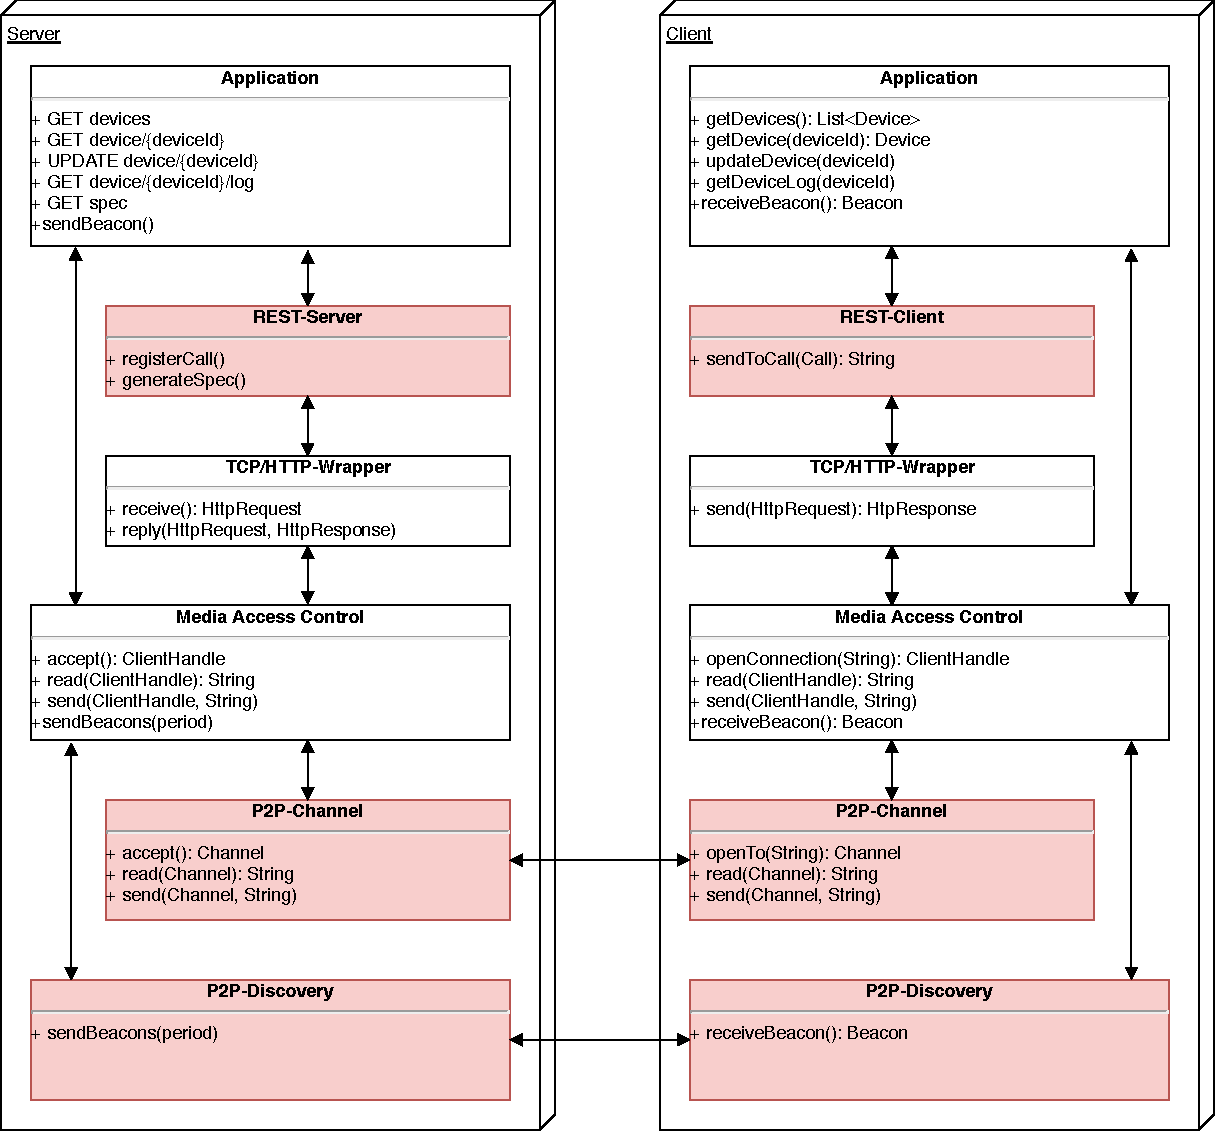
\includegraphics[width=0.85\textwidth]{IOT-Connectivity-Protocol-Stack}
    	\caption{Zu sehen sind die Schnittstellen, die nötig sind, um die Client-Server Anwendung über p2p nutzen zu können. Hierbei stehen alle rot hinterlegten Schnittstellen bereits zur Verfügung. Wenn die genutzte p2p Schnittstelle es nicht erlaubt, TCP/HTTP Pakete an die Ports einer Netzwerkschnittstelle des Servers zu senden, muss ein TCP/HTTP-Wrapper erstellt werden. Andernfalls besteht die Implementierung aus einem gewöhnlichem REST-Client/Server-Paar. Getrennt davon muss jedoch auch innerhalb der Anwendung die p2p-Service-Discovery angebunden werden. }
	    \label{protocol_stack}
	\end{figure}     
    
    \section{Umsetzung}
	Um eine stabile Lösung schnell und simpel anbieten zu können, wird zur Implementierung der REST-Schnittstelle auf bestehende Server sowie Client Bibliotheken zurückgegriffen. Diese bieten somit die Möglichkeit die Implementierung dieser Schnittstelle deskriptiv vorzunehmen. In Android wird somit die Implementierung zur Laufzeit aus einer Schnittstellenbeschreibung generiert und auf der Serverseite müssen so nur die Implementierungen der Methoden beschrieben werden. Da die Wahl des Übertragungsmediums auf WiFi-Direct gefallen ist, können ebenso Teile des Betriebssystems und Standardbibliotheken zum Broadcast und Aufbau der p2p Verbindung genutzt werden.
	Da unter Linux das Paket wpa\_supplicant \cite{wpaSupplicant} auf allen gängigen Distributionen, so auch unter raspbian auf dem Raspberry Pi, dazu genutzt wird, WiFi Schnittstellen und Netzwerke zu verwalten. Es läuft als daemon im Betriebssystem mit und kann über ein Kommandozeileninterface bedient werden oder mit einer C-Schnittstelle in das eigene Programm eingebunden werden.
	\subsection{Pharo}
		Auf der Serverseite in Pharo besteht die Implementierung aus der Anbindung der wpa\_supplicant Schnittstelle, einem C-Modul für diese Anbindung, den Methoden des REST-Servers und einem Modul, welches die p2p Verbindung und Service Discovery handhabt.
		Die Anbindung des wpa\_supplicant beginnt damit, dass aus der hostap \cite{hostAp} Bibliothek ein C-Modul kompiliert werden muss, welches es erlaubt, das interne Control Interface (common/wpa\_ctrl.c) zu nutzen. Darauf aufbauend muss in pharo eine Klasse geschaffen werden, die in der Lage ist, Handle (LWpaHandle) des Control Interfaces zu verwalten und deren Zustand persistent zu speichern. Persistenz ist nötig, da die pharo-VM zwischen Nachrichten gestoppt und zu einem anderen Zeitpunkt erst wieder fortgesetzt werden kann. Wenn verwendete Netzwerkschnittstellen vom Gerät entfernt werden, muss dies dann auch aus der Bibliothek als Fehler signalisiert werden. Weiterhin müssen Events über Polling an Listener signalisiert werden und außerhalb des wpa\_supplicant kann die Liste der verfügbaren Schnittstellen abgefragt werden.
		
		Basierend auf dieser Anbindung wird LWpaInterface als einheitliche Fassade genutzt, die alle genutzten Nachrichten, die an den wpa\_supplicant gesendet werden können, als Methoden implementiert.
		In diesem Interface sind alle Methoden der p2p Service Discovery über p2p Verbindungsaufbau und Netzwerkscans bis hin zur Netzwerkkonfiguration enthalten. Alle Methoden stehen auch auf allen Netzwerkgeräten zur Verfügung, es ist aber zu erwarten, dass bei nicht unterstützten Methoden ein Fehler auftritt.
		Die p2p Komponente, welche Service Discovery und p2p Verbindungsaufbau ermöglicht, ist ein einzelnes Objekt, welches über start und stop Methoden verfügt, um die Softwarelösung als gebündelte Einheit zu betreiben. Dieses Objekt startet auch gleichzeitig den REST-Server auf einem definierten Port, da dieser Port in der p2p Service Discovery angegeben werden muss, damit Clients den Server auch nutzen können. Weiterhin sind für WiFi Direct Event Handler nötig, die auf Events zum Verbindungsaufbau reagieren und Verbindungen akzeptieren.
		
		Zur Implementierung des REST-Servers müssen die Methoden, die der REST-Server anbieten soll, als Kinder einer Abstraktenklasse (ICCall) definiert werden, sodass die Liste der Kinder dem REST-Server zugeliefert werden kann.
		Jede Klasse beschreibt dabei einen Pfad des Servers auf dem ein oder mehrere Http-Verben implementiert werden. Da manche Methoden jedoch auf anderen Methoden aufbauen, wird zwischen der wpa\_supplicant Bibliothek und der Methodenimplementierung eine Logikschicht (IC...Wrapper) eingebaut, welche es erlaubt, die noch nicht in JSON umgewandelten Resultate (ICData) in mehreren REST-Methoden abzufragen.
		
	\subsection{Android}

		Die Android App besteht aus zwei Modulen, einem Frontend, welches die anzuzeigenden Daten über RxJava asynchron abfragt und einem Modul, welches die p2p Broadcasts abfragt sowie die p2p Verbindung aufbaut.
		Die App besteht aus einer Reihe einfacher Bildschirme, die größtenteils bloß Listen der abgefragten Daten anzeigen. Wie in \figurename \ref{protocol_stack} zu sehen, ist der Nutzerfluss durch die Bildschirme, dass der Nutzer zunächst eine Liste der in der Nähe aktiven p2p Geräte angezeigt bekommt und eines dieser Geräte auswählt. Durch die Auswahl wird eine p2p Verbindung mit dem Gerät aufgebaut, sodass der REST-Server genutzt werden kann. Während der Nutzer einen Ladebildschirm sieht, wird so die Liste der verfügbaren Netzwerkschnittstellen, die nicht exklusiv für p2p vorhanden sind, abgefragt und dem Nutzer angezeigt. Sollte diese Liste nur einen Eintrag enthalten, wird die Auswahl der Netzwerkschnittstelle automatisch vorgenommen und es wird zur nächsten Ansicht vorrangeschritten. Der Nutzer sieht hierbei nach wie vor den Ladebildschirm. Sind jedoch mehrere Elemente in der Liste, wird dem Nutzer die Liste angezeigt. Wählt der Nutzer eine der Netzwerkschnittstellen aus, wird ihm eine Liste der aktuell erreichbaren Netzwerke gezeigt, sodass er das Gerät mit Netzwerken verbinden kann, wie es auch in den Einstellungen des Smartphones möglich ist.
		
		Um die Module miteinander zu verbinden, wird Koin \cite{androidKoin} als Dependency Injection in Verbindung mit öffentlich definierten Schnittstellen genutzt. Koin verzichtet im Gegensatz zu Dagger auf generierten Code. Dadurch ist es zwar im Setup langsamer, jedoch macht es für die eigentliche Injection der Abhängigkeiten keinen erheblichen Unterschied mehr, sodass diese Bibliothek auf Grund ihrer leichten Einbindung genutzt wurde \cite{androidKoinSpeed}. Als REST-Client wird hierbei Retrofit in Kombination mit Gson genutzt. Retrofit erlaubt es, die REST-Schnittstelle deklarativ zu definieren, sodass jeglicher Code generiert wird. Dies hat den Vorteil, das kein Boilerplate-Code geschrieben werden muss. In Verbindung mit Gson lässt sich so eine saubere REST-Schnittstelle mit einem klar strukturierten Datenmodell umsetzen, da gson es erlaubt, Datenobjekte aus Klassen zu erzeugen, in denen die Felder mit dem gelieferten JSON Objekt korrespondiert.

	\subsection{Stolpersteine}
		Bei der Umsetzung des Projektes sind einige unvorhergesehene Probleme und Einschränkungen aufgetaucht. Teilweise erforderten diese ein großes Umdenken oder eine lange Suche nach einer alternativen Lösung.
		
		Die Kommandozeilenschnittstelle	des wpa\_supplicant ist dem C-Interface unterlegen, da Events immer im Standardkanal ausgegeben werden. Dies führt dazu, dass bei der Nutzung von Befehlen nicht zwischen eingehenden Events und dem Ergebnis des Befehls unterschieden werden kann. Die C-Schnittstelle erlaubt es hingegen, Events unabhängig von Befehlen abzufragen und auf Diese zu warten. Foreign Function Calls sind in pharo zwar aktuell möglich, jedoch sind diese noch nicht vollständig eingebunden. So wird aktuell noch die gesamte Ausführung in der VM für die Dauer des externen Aufrufes gestoppt, da nicht überblickt werden kann, inwie weit der externe Aufruf Speicherveränderungen durchführt und somit Inkonsistenzen entstehen könnten. Außerdem ist es zum aktuellen Zeitpunkt nicht möglich, mit dem Unified Foreign Function Interface (UFFI) in pharo Callbacks zu Implementieren. Dies bedeutet konkret, dass Events lediglich über ein Polling erhalten werden müssen.
		Weiterhin ist UFFI noch nicht so gut dokumentiert, dass es ohne viele Vermutungen ausprobiert werden muss. Es wurde sich hierbei zwar an bereits bestehendem Code der git Anbindung orientiert, jedoch ist es teilweise undurchsichtig, welche Typen von der VM automatisch übersetzt werden, wie zum Beispiel char* zwar zu String umgewandelt wird, dies jedoch nicht wie ein Stringbuffer funktioniert.
		
		Beim Testen von UFFI besteht das Problem, dass die Aufrufe, die aus pharo getätigt werden, in einem core dump resultieren, falls ein Fehler auftritt und so nicht gespeicherte Änderungen in der VM verloren gehen. Da hierbei viel mit sehr generischem Code gearbeitet wird, der das Stringarray aus pharo, welches den C-Funktionsaufruf repräsentiert, in einen tatsächlichen Funktionsaufruf umwandelt. Dadurch ist der stacktrace des Codes, der nativ ausgeführt wird, wenig durchsichtig und man bleibt ohne Fehlermeldung dessen, was tatsächlich schief gelaufen ist. Dies ist besonders problematisch im Hinblick darauf, dass die Typauflösung von UFFI nicht ganz deutlich wurde und man somit auf Trial and Error zurückgreifen musste.
		
		Theoretisch blockieren sich die Verwendung von WiFi-Direct und gewöhnlichem WiFi mit einem Access Point auf der selben Netzwerkschnittstelle, da diese eine Sende- und Empfangseinheit exklusiv benötigen. Diese Limitierung wird bei Nutzung des wpa\_supplicant jedoch nicht deutlich, da gewöhnliche Schnittstelle und p2p Schnittstelle immer als separate Einheiten auf der gleichen Netzwerkkarte aufgelistet werden. Da manche Netzwerkkarten inzwischen mehr als ein Radio enthalten, um höhere Übertragungsraten zu ermöglichen, kann dies jedoch auf manchen Geräten dennoch funktionieren. Im Falle des Raspberry Pi 3 B ist dies jedoch aktuell nicht möglich und eine zweite Netzwerkkarte wird benötigt, um WiFi Direct und WiFi parallel zu nutzen. Diese Limitierung gilt jedoch nicht für die Service Discovery, die über WiFi Direct stattfindet.
		
		Im Allgemeinen ist die Dokumentation und Spezifikation von WiFi Direct und dessen Implementierung unzureichend. Die Spezifikation konnte von der WiFi Association nicht angefragt werden, somit fehlt sie für dieses Projekt. Da so einzig die Dokumentation des wpa\_supplicant für die Umsetzung genutzt werden konnte, fielen auch hier Lücken auf. So sind nicht alle relevanten Events dokumentiert und es ist noch fraglich, ob die genutzten Events tatsächlich das widerspiegeln, was ihr Name suggeriert. Ebenso fehlt ein State-Graph der p2p Umsetzung, wodurch unklar ist, in welchem Zustand des Verbindungsaufbaus die Netzwerkpartner sich wie zu verhalten haben. Außerdem fehlen Angaben zu den Datagrammen der Service Discovery in der Dokumentation, da Diese direkt binär codiert angegeben werden müssen. Es wurde hierbei auf die Open Source Android Implementierung zurückgegriffen.\cite{androidRepo}
		
		Unter Android steht WiFi Direct vom Betriebssystem als Sammlung von Java Klassen zur Verfügung. Problematisch ist hierbei auch wieder, dass Android oder der intern verwendete wpa\_supplicant einen Cache besitzt, wodurch Daten, die bereits einmal ausgeliefert wurden trotz einer neuen Anfrage nicht noch einmal ausgeliefert werden. Ebenso scheint es eine Blacklist für Geräte zu geben, zu denen ein p2p Verbindungsaufbau mehrfach fehlgeschlagen ist, wodurch auch kein Service Discovery Austausch mehr mit diesem Gerät möglich ist. Dieses Problem ließ sich lediglich durch einen Neustart des Smartphones beheben.
		
		Aus all diesen Faktoren resultiert, dass die Verbindung nicht reproduzierbar stabil zwischen dem Raspberry Pi und einem Android Smartphone aufgebaut werden kann, wodurch eine Nutzbarkeit für Endnutzer hinfällig wird.
    
    \begin{figure}[ht]
		\centering
	    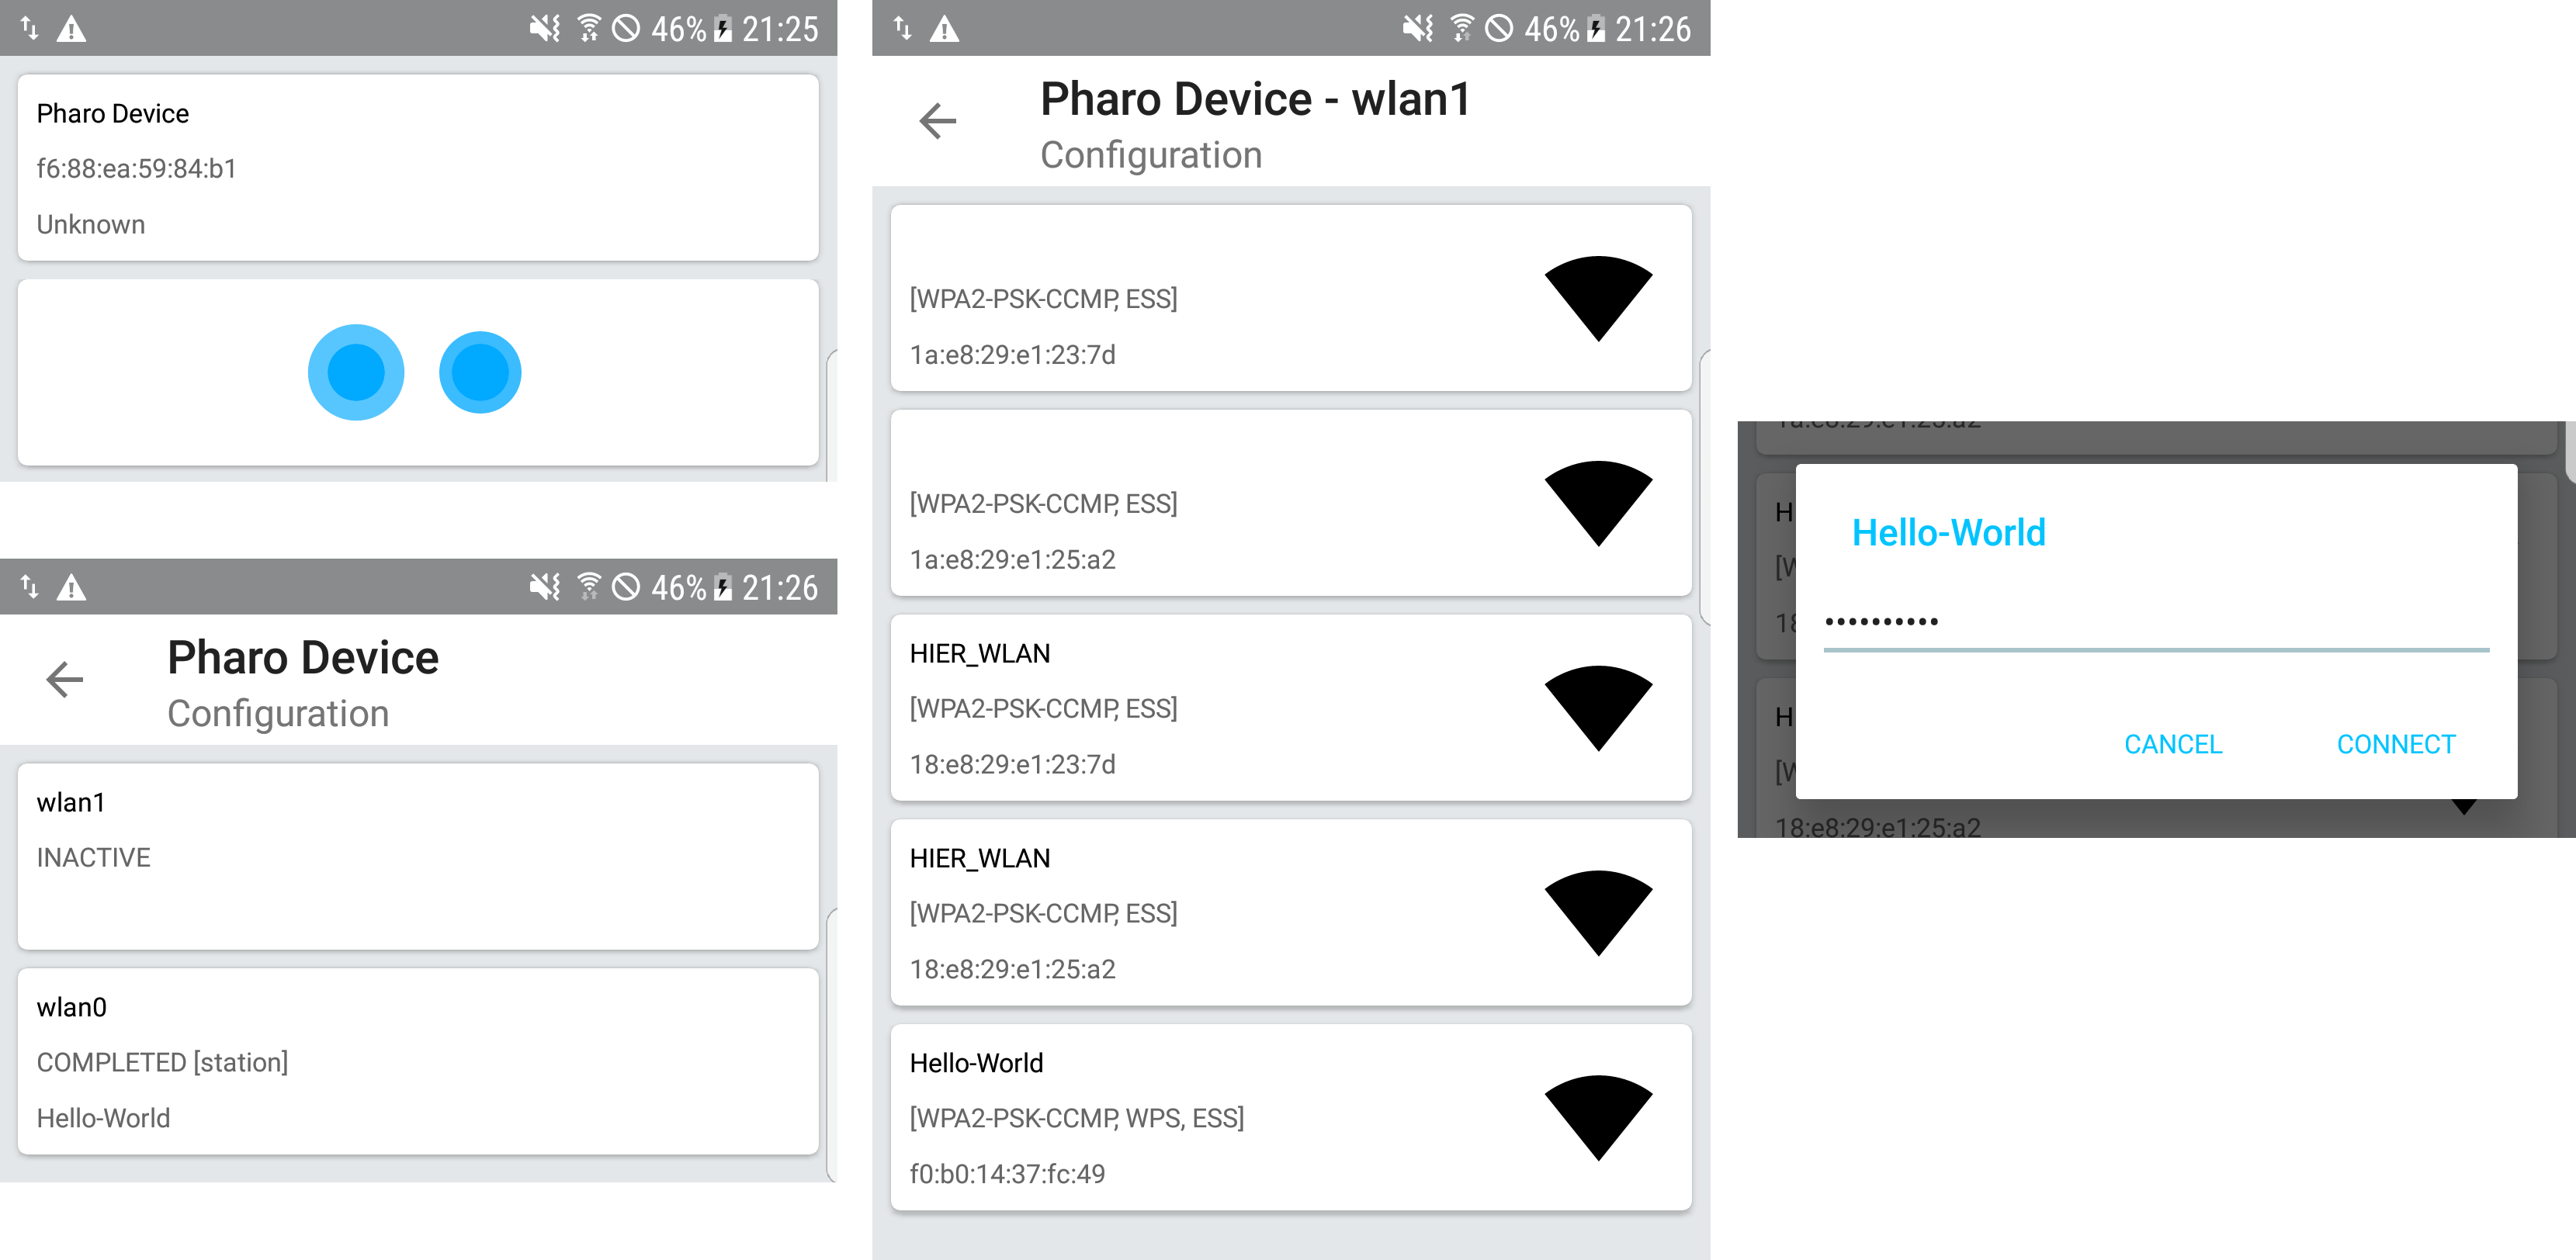
\includegraphics[width=0.95\textwidth]{user_flow.png}
    	\caption{ Der Benutzer sieht zunächst eine Liste an konfigurierbaren Geräten in der Nähe (links oben), durch Auswahl bekommt der Nutzer die Liste der verfügbaren Netzwerkschnittstellen zu sehen (links unten). Sobald auch hier eine Auswahl erfolgt ist, kann der Nutzer eine Liste an verfügbaren und bereits kofigurierten Netzwerken für diesen Netzwerkadapter sehen (mitte). Letztlich kann der Nutzer noch ein Netzwerk durch Eingabe des Passworts konfigurieren (rechts). }
	    \label{protocol_stack}
	\end{figure}
	
	\pagebreak
	\section{Ausblick}
	Im Rahmen dieses Projektes wurde Wi-Fi Direct zur Nutzung als p2p Technologie zwischen Android und pharo untersucht. Zwecks mangelnder Dokumentation von Wi-Fi Direct und dessen Implementierung unter Linux war es nicht möglich, eine stabile Verbindung wiederholbar aufzubauen. Da Service Discovery jedoch größtenteils stabil über Wi-Fi Direct funktioniert, ist zu überlegen, ob eine Hybrid Lösung in Verbindung mit Bluetooth oder anderen p2p Technologien sinnvoll ist. Damit wäre es möglich, manche Nachteile von anderen Technologien auszugleichen. In Kombination mit Bluetooth könnte so die Broadcastreichweite spürbar erhöht werden. Generell sollten somit andere Technologien auch auf deren Nutzbarkeit überprüft werden. Für Diese wird es dann auch nötig, einen Wrapper um Socketverbindungen zu bauen.
	Ebenso ist es denkbar, mehrere p2p Technologien parallel zu betreiben, damit der Nutzer nicht durch eine fehlende Technologie in seinem Smartphone eingeschränkt wird. Hierbei sollte auch darauf geachtet werden, dass der Nutzer nicht von dieser Parallelität behelligt wird, somit die Auswahl automatisch geschieht.
	
	Der implementierte REST-Server verwendet noch den standardmäßigen Error Handler, der im Fehlerfall einen Stacktrace als plain text zurückliefert. Dies sollte abgefangen werden und in ein JSON Objekt mit Fehlercodes und sprechenden Fehlermeldungen umgewandelt werden. Aktuell führt der REST-Server noch alle Aufrufe ohne Authentifizierung durch. Es sollte jedoch wenigstens eine Authentifizierung bei der Erstkonfiguration festgelegt werden, sodass nicht autorisierte Personen keine Änderungen an den Einstellungen vornehmen können.
	In Verbindung mit dieser Authentifizierung auf Anwendungsebene kann auch das Gerät an ein virtuelles Netzwerk gebunden werden, welches eigene Geräte bündelt. Dieses virtuelle Netzwerk wird dazu genutzt, dass die Geräte einen Server in diesem Netzwerk besitzen, auf den sie sich beziehen können. Dies kann entweder eine lokal laufende pharo Instanz sein oder ein Cloudservice, an dem das virtuelle Netzwerk einem Account entspricht. Damit wird nicht nur der Zugriff lokal sondern auch Remote eingeschränkt. Um diese virtuellen Netzwerke gut verwalten zu können, empfiehlt es sich auch hierbei ein DNS Service Discovery einzusetzen, die Daten jedoch durch verschiedene Maßnahmen zu schützen.\cite[S.8]{Kaiser2}
	
	Im Rahmen von Low Energy Netzwerken könnten die Broadcasts der Service Discovery von anderen pharo Instanzen auch erkannt werden und so gebündelt werden. Dies erlaubt es, Energie dadurch einzusparen, dass nur noch ein Gerät aus dem Low Energy Netzwerk den Broadcastanfragen antworten muss. Ebenfalls lässt sich so die Reichweite von p2p Verbindungen erhöhen, da die Anfragen zum entsprechenden Ziel weitergeleitet werden können. Im Hinblick auf Bandbreite stellt dies erst ein Problem dar, wenn mehrere Geräte im selben Netzwerk parallel administriert werden, was jedoch einen Randfall darstellen sollte und somit vorerst ignoriert werden kann. Es ist somit also denkbar die pharo Instanzen als Knoten in einem Netzwerk aus oben genannten Gründen agieren zu lassen. Diese Knoten müssten dann jedoch ebenfalls Routingtabellen verwalten, was dieses dezentrales Netzwerk im Vergleich zum Nutzen, der daraus gewonnen wird, zu kompliziert macht.
	
	

    \begin{thebibliography}{10}
        \bibitem[Aneja et al.]{Aneja}Nagender Aneja und Sapna Gambhir: "Profile-Based Ad Hoc Social Networking Using Wi-Fi Direct on the Top of Android" {\it Mobile Information Systems, Volume 2018, Article ID 9469536, 7 pages} (2018).
        \bibitem[Eberhardt et al.]{Kelm} Udo Eberhardt und Hans Joachim Kelm [Hrsg.]: {\it USB - Universal Serial Bus} Franzis, Poing (1999).
        \bibitem[Esnaashari et al.]{Esnaashari} Shadi Esnaashari, Ian Welch und Peter Komisarczuk: {\it Determining home users' vulnerability to Universal Plug and Play (UPnP) attacks} Erschienen in: Proceedings of the 2013 27th International Conference on Advanced Information Networking and Applications Workshops (WAINA). IEEE, 2013. - S. 725-729. - ISBN 9781467362399 .
        \bibitem[Kaiser et al.]{Kaiser} Daniel Kaiser, Marcel Waldvogel, Holger Strittmatter und Oliver Haese: {\it User-Friendly, Versatile, and Efficient Multi-Link DNS Service Discovery} Erschienen in: Proceedings 2016 IEEE 36th International Conference on Distributed Computing Systems Workshops : ICDCSW 2016. - Piscataway, NJ : IEEE, 2016. - S. 146-155. - ISBN 978-1-5090-3686-8.
        \bibitem[Kaiser, Waldvogel]{Kaiser2} Daniel Kaiser und Marcel Waldvogel: {\it Adding Orivacy to Multicast DNS Service Discovery} Erschienen in: Proceedings - 2014 IEEE 13th International Conference on Trust, Security and Privacy in Computing and Communications (TrustCom) ; Beijing, China, 24 Sep - 26 Sep 2014. - Piscataway : IEEE, 2014. - S. 809-816. - ISBN 978-1-4799-6513-7.
        \bibitem[Langer et al.]{Langer}Josef Langer und Michael Roland: {\it Anwendungen und Technik von Near Field Communication (NFC)} Springer, Heidelberg (2010).
        \bibitem[Lüders]{Lueders}Christian Lüders: {\it Lokale Funknetze: Wireless LANs (IEEE 802.11), Bluetooth, DECT} Vogel, Würzburg (2007).
        \bibitem[Morrow]{Morrow}Robert Morrow: {\it Bluetooth Operation and Use} McGraw-Hill (2002).
        \bibitem[Sauter]{Sauter}Martin Sauter: {\it Grundkurs Mobile Kommunikationssysteme: LTE-Advanced, UMTS, HSPA, GSM, GPRS, Wireless LAN und Bluetooth} 6.Auflage Springer Vieweg, Wiesbaden (2015).
        \bibitem[Sikora]{Sikora}Axel Sikora: {\it Wireless LAN: Protokolle und Anwendungen} Addison-Wesley, München u.A. (2001).
		\bibitem[Townsend et al.]{Townsend} Kevin Townsend, Carles Cuffí, Akiba und Robert Davidson: {\it Getting Started with Bluetooth Low Energy} O'Reilly (2014).
		
		\bibitem[Android Koin]{androidKoin}https://insert-koin.io/
		\bibitem[Android Koin Speed]{androidKoinSpeed}https://medium.com/koin-developers/ready-for-koin-2-0-2722ab59cac3
        \bibitem[Android Open Accessory]{AOA}https://source.android.com/devices/accessories/custom
        \bibitem[Android OkHttp Repository]{AndroidOkHttp}https://github.com/square/okhttp
        \bibitem[Android Permissions]{androidRights}https://elinux.org/Android\_Security\#Paranoid\_network-ing
        \bibitem[Android Repository]{androidRepo}https://android.googlesource.com/platform/frameworks/base
        \bibitem[iot-p2p-test Repository]{test-repository}https://github.com/janphkre/iot-p2p-test
        \bibitem[JSON Schema]{JsonSchema}https://json-schema.org/
        \bibitem[Linux Packet]{linuxPacket}http://man7.org/linux/man-pages/man7/packet.7.html
        \bibitem[OpenAPI]{OpenApi}https://swagger.io/docs/specification/about/
        \bibitem[Pharo]{pharo}http://pharo.org/
        \bibitem[Pharo OpenAPI Fepository]{pharoOpenApi}https://github.com/zweidenker/openapi
        \bibitem[Pharo Things Repository]{pharoThings}https://github.com/pharo-iot/PharoThings
        \bibitem[Pharo Zinc Repository]{pharoZinc}https://github.com/zweidenker/zinc/
        \bibitem[WiFi Direct]{wifiDirect}https://www.wi-fi.org/discover-wi-fi/wi-fi-direct                        		\bibitem[WiFi HostAP Repository]{hostAp}git://w1.fi/hostap.git
        \bibitem[WiFi wpa\_supplicant]{wpaSupplicant}https://w1.fi/wpa\_supplicant/
        \bibitem[Zweidenker]{zweidenker}https://zweidenker.de
    \end{thebibliography}
\end{document}
